%
% This work is licensed under a Creative Commons Attribution-ShareAlike 4.0 International License.
%

\documentclass[10pt, letterpaper, twoside, openany]{article}

\title{Introduction to Quantum Mechanics -- Worksheet 1}
\author{Joseph D. MacMillan}
\date{}


\usepackage{graphicx}
\usepackage{color} 
\usepackage{amsmath, amssymb}
\usepackage{libertinus}
\usepackage{microtype}
\usepackage{layout}
\usepackage[most]{tcolorbox}
\tcbuselibrary{skins,breakable}
\usepackage[hang, small, bf]{caption}
\captionsetup[table]{position=top}
\captionsetup[figure]{position=bottom}
\usepackage[hyphens]{url}
\usepackage[hidelinks]{hyperref}
\hypersetup{pdftitle={Introduction to Quantum Mechanics -- Worksheet 1}}
\hypersetup{pdfauthor={Joseph D. MacMillan}}
\urlstyle{rm}
\usepackage[shortlabels]{enumitem}
\usepackage[margin=1in]{geometry}
\usepackage{fancyhdr}




\newcommand{\uu}{\symbfup{u}}
\newcommand{\grad}{\symbfup{\nabla}}
\newcommand{\curl}{\symbfup{\nabla} \times}
\newcommand{\dfdx}[2]{\frac{\partial {#1}}{\partial {#2}}}
\newcommand{\ddfdx}[2]{\frac{\partial^2 {#1}}{\partial {#2}^2}}
\newcommand{\vort}{\symbfup{\omega}}
\renewcommand\vec{\symbfup}
\newcommand{\unit}[1]{\hat{\vec{#1}}}
\newcommand{\U}{\mathbb{U}}
\newcommand{\V}{\mathbb{V}}
\newcommand{\LL}{\mathbb{L}^2}
\newcommand{\LLLL}{\mathbb{L}^4}

\newcommand{\ket}[1]{| #1 \rangle}
\newcommand{\bra}[1]{\langle #1 |}
\newcommand{\braket}[2]{\langle #1 | #2 \rangle}


%\DeclareMathAlphabet{\mathbfsf}{\encodingdefault}{\sfdefault}{bx}{sl}
\newcommand{\tens}[1]{\mathbfsfit{#1}}


\newcounter{example}[section]
\def\theexample{\thechapter.\arabic{example}}
\newenvironment{example}[1][ ]{\refstepcounter{example}
\begin{tcolorbox}[breakable, sharp corners, boxrule = 0pt, frame empty, opacityframe=0, parbox=false]
\textbf{Example \theexample \ -- #1.}
}
{ 
\end{tcolorbox}
}

\newenvironment{theorem}[1][ ]{
\begin{tcolorbox}[breakable, sharp corners, boxrule = 0pt, frame empty, opacityframe=0, parbox=false]
\textbf{#1.}
}
{ 
\end{tcolorbox}
}

\newcounter{problem}[section]
\def\theproblem{\thechapter.\arabic{problem}}
\newenvironment{problem}[1][ ]{\refstepcounter{problem} \noindent \textbf{Problem \theproblem \ -- #1.}}{\vspace{0.1in}}


\begin{document}

\pagestyle{fancy}
\fancyhead[L]{\emph{Introduction to Quantum Mechanics}}
\fancyhead[R]{Worksheet 1} 

\Large \noindent Worksheet 1

\noindent \LARGE \textbf{Stern-Gerlach and Quantum States}

\normalsize

\vspace{0.2in}

\noindent Exploring the Stern-Gerlach Experiment  \bullet \  Kets and Bras   \bullet \  Normalization   \bullet \  Inner Products  

\vspace{0.1in}

\noindent \rule{\textwidth}{0.5pt}

\vspace{0.2in}

\begin{enumerate}
\item This question uses the SPINS simulation which you can find online at \url{https://physics.weber.edu/schroeder/software/Spins.html}.  First, set up the Stern-Gerlach experiment so that it matches the image below: 
\begin{center}
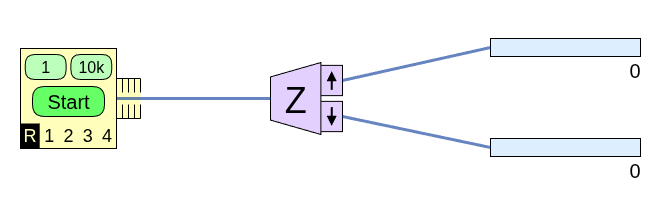
\includegraphics[scale=0.4]{fig1.png}
\end{center}

\begin{enumerate}
\item Play a bit with the experiment -- keep the ``oven'' on R (for random) so that the particles come out thermalized (with randomly pointing $\mathbf{S}$ vectors), but try firing one particle at a time or 10,000 at a time.  Then reset and just send one particle through over and over -- maybe 20 times in total.  Then answer the following questions.

{Can you predict the spin measurement outcome (spin up or spin down) when you send a single particle in?} 

\vspace{1.5in}

{After sending in 20 particles, can you predict \emph{exactly} how many would be counted in each output counter?}

\vspace{1in}

\item If you ran the experiment for 10,000 particles, and you observed 4,950 spin up and 5,050 spin down counts, would you argue that something funny is going on (perhaps the initial state has been prepared in configuration that is \emph{not} ``50/50'' after all?) Or would you simply call it statistical fluke?  Why?  What if it came out 4,800 spin up?  How about 4,000? 

\newpage

\item Consider flipping a coin:  we expect on average 50\% heads and 50\% tails, and the \emph{standard deviation} (or \emph{uncertainty}) will be on the order of $\sqrt{N}$, where $N$ is the number of coin tosses.  Revisit the last question with this in mind; how far off from 50/50 can the results be before you get suspicious?

\end{enumerate}

\vspace{1.5in}

\item Next, consider a ``chained'' Stern-Gerlach experiment with two unknown analyzers as shown below.
\begin{center}
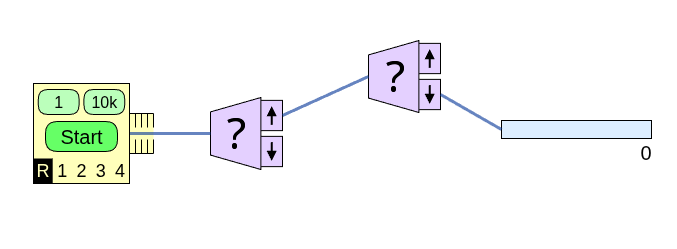
\includegraphics[scale=0.4]{fig2.png}
\end{center}

\begin{enumerate}
\item Suppose you hit the 10k button, sending 10,000 particles through the experiment.  What is the maximum possible value (approximately) that would be counted?  What about the minimum?  Feel free to set up the experiment yourself to see.

\vspace{1.5in}

\item Suppose the second analyzer is oriented along the $z$ direction.  Then you send in just one particle, and that particle ends up being detected at the counter.  What can you conclude about what the first analyzer must be (or what it must not be)?

\end{enumerate}

\newpage

\item Consider these different spin-1/2 states, given in Dirac notation by
\begin{align*}
\ket{\psi_1} &= 3 \ket{+} + 4\ket{-} \\
\ket{\psi_2} &= \ket{+} + 2i \ket{-}
\end{align*}
\begin{enumerate}
\item Normalize each state.

\vspace{2in}

\item Write each state in matrix notation.

\vspace{2in}

\item Write the bra of each ket; write the bras in matrix notation, too.

\newpage

\item Find a (normalized) ket that is orthogonal to each state.

\vspace{4in}

\item Compute the following inner products, using either Dirac notation or matrix notation:  $\braket{\psi_1}{\psi_2}$, $\braket{\psi_2}{\psi_1}$.
\end{enumerate}

\end{enumerate}

\end{document}
